\chapter{Il tool DDoShield}

In questo capitolo verrà presentato ed analizzato il tool DDoShield, uno strumento avanzato progettato per supportare la ricerca e lo sviluppo dei sistemi di rilevamento delle intrusioni (IDS) nell'ambito dell'Internet of Things (IoT). DDoShield è una piattaforma di simulazione che utilizza container Docker e il simulatore di rete NS-3 per generare e catturare traffico di rete realistico, sia benigno che malevolo. L'obiettivo principale di DDoShield è facilitare lo sviluppo, il test e la valutazione degli IDS specifici per le reti IoT, affrontando la necessità di dataset di alta qualità e la mancanza di piattaforme realistiche per simulare scenari di attacco.

\section{Presentazione di DDoShield}

DDoShield è nato dalla necessità di creare un ambiente di test realistico per la valutazione degli IDS progettati per le reti IoT. Le reti IoT, grazie alla loro crescente adozione in settori come la casa intelligente, le città intelligenti, la sanità e i veicoli autonomi, presentano una superficie di attacco sempre più estesa. Questo incremento ha reso le reti un obiettivo primario per cyber-attacchi, in particolare per gli attacchi DDoS (Distributed Denial of Service) che sfruttano botnet per sovraccaricare i dispositivi connessi. Gli IDS per IoT sono strumenti fondamentali per identificare e mitigare tali minacce, ma devono essere progettati tenendo conto delle risorse limitate dei dispositivi IoT e delle caratteristiche particolari delle reti in cui operano.

DDoShield si distingue dagli altri testbed per la sua capacità di generare traffico di rete realistico e di supportare l'implementazione di diversi modelli di machine learning per il rilevamento in tempo reale degli attacchi botnet DDoS. Sfrutta il simulatore di rete NS-3 per creare una rete simulata, all'interno della quale sono ospitati sia IDS che applicazioni IoT tramite container Docker. Questa architettura permette a DDoShield di simulare scenari IoT dettagliati, migliorando il realismo e l'efficacia dei test.

Una delle innovazioni principali di DDoShield è la capacità di generare traffico sia benigno che malevolo. Il traffico benigno include dati di trasferimento file \textbf{(FTP)}, streaming video \textbf{(RTMP)} e traffico \textbf{HTTP}, mentre il traffico malevolo è rappresentato dai dati generati dal \textbf{malware Mirai}, noto per i suoi attacchi DDoS su dispositivi IoT.

\section{Architettura del sistema}

DDoShield è costruito sulla base del tool preesistente DDoSim, progettato per simulare attacchi DDoS di larga scala nell'ambito IoT. Mentre DDoSim si concentra sulla simulazione degli attacchi, DDoShield estende queste capacità integrando sia traffico benigno che malevolo e includendo la possibilità di valutare gli IDS attraverso diversi modelli di machine learning, come il Random Forest \textbf{(RF)}, il \textbf{K-Means} e la rete neurale convoluzionale \textbf{(CNN}). Questo rende DDoShield una piattaforma completa per lo sviluppo, il test e l'analisi degli IDS in un ambiente realistico e controllato.\cite{DDoSim}

L'infrastruttura di DDoShield si basa su Docker, una piattaforma open-source che permette di creare e gestire applicazioni all'interno di container isolati. Ogni componente dell'attacco DDoS, come l'attaccante e i dispositivi compromessi (Devs), è simulato all'interno di container Docker, questi interagiscono attraverso una rete simulata creata con NS-3. Questa configurazione implementativa permette di replicare dinamiche di rete reali e testare le risposte degli IDS in un ambiente controllato, senza dover gestire la complessità fisica di una rete IoT reale.

\section{Funzionalità principali}

Una delle funzionalità più significative di DDoShield è la sua capacità di integrare traffico di rete realistico sia benigno che malevolo, permettendo così di testare e valutare gli IDS in un ambiente che simula accuratamente scenari reali. Questo è particolarmente importante nel contesto IoT, dove i dispositivi hanno risorse limitate e le reti sono eterogenee e dinamiche. DDoShield consente la generazione di due categorie principali di traffico:

\begin{itemize}
    \item \textbf{Traffico benigno}: Generato da server reali simulati, come Apache, Nginx e un server FTP personalizzato. Questi server producono il traffico di attività normali in un ambiente IoT. Questo tipo di traffico è essenziale per fornire un punto di riferimento con cui gli algoritmi di rilevamento delle intrusioni possono confrontare il traffico anomalo. La varietà di traffico generata consente di evitare dataset sbilanciati e di migliorare l’adattabilità degli IDS a scenari complessi.
    \item \textbf{Traffico malevolo}: Simulato utilizzando il malware Mirai, uno dei più noti strumenti utilizzati per gli attacchi botnet DDoS su dispositivi IoT. Tra gli attacchi DDoS simulati vi sono il SYN Flood, l'ACK Flood e l'UDP Flood, tutti progettati per sovraccaricare i server bersaglio con un volume elevato di richieste, impedendo loro di operare normalmente. Questi attacchi sono scelti appositamente per testare le capacità di rilevamento degli IDS in un ambiente simulato realistico.
\end{itemize}

DDoShield non solo permette di simulare questi attacchi, ma consente anche l'implementazione e la valutazione di IDS basati su modelli di machine learning. L'IDS in DDoShield è in grado di rilevare attacchi botnet DDoS in tempo reale, sfruttando tre diversi algoritmi:

\begin{itemize}
    \item \textbf{K-Means}: Un algoritmo di clustering non supervisionato che divide il traffico di rete in gruppi distinti. L'obiettivo è identificare automaticamente i pattern anomali nel traffico senza la necessità di dataset pre-etichettati. Questo lo rende particolarmente utile in ambienti in cui i dati non sono sempre chiaramente classificati.
    \item \textbf{Random Forest (RF)}: Un algoritmo supervisionato che utilizza una combinazione di alberi decisionali per classificare il traffico come benigno o malevolo. La sua forza risiede nella capacità di ridurre l'overfitting e migliorare la generalizzazione delle previsioni.
    \item \textbf{Reti neurali convoluzionali (CNN)}: Un potente strumento di deep learning che non richiede un'estrazione manuale delle feature dal traffico di rete. Le CNN sono particolarmente efficaci nel rilevare pattern complessi e non lineari, rendendole ideali per la rilevazione delle anomalie nelle reti IoT.
\end{itemize}

Questi modelli di machine learning sono implementati all'interno di container Docker e sono in grado di analizzare il traffico di rete in tempo reale, fornendo una classificazione istantanea tra traffico benigno e malevolo. La capacità di utilizzare modelli diversi consente una valutazione comparativa delle performance, permettendo ai ricercatori di scegliere l'algoritmo più adatto alle loro esigenze specifiche.

\section{Componenti del sistema}

Il framework DDoShield è costituito da quattro principali componenti, tutti ospitati all'interno di container Docker, che interagiscono tra loro attraverso una rete simulata creata con NS-3:

\begin{enumerate}
    \item \textbf{Attaccante (Attacker)}: Questa entità coordina l'attacco DDoS, sfruttando le vulnerabilità dei dispositivi Devs per diffondere il malware della botnet. Utilizza un insieme di script di exploit e infezione per compromettere i dispositivi e farli partecipare agli attacchi.
    \item \textbf{Dispositivi compromessi (Devs)}: Rappresentano dispositivi vulnerabili connessi alla rete IoT, compromessi dall'attaccante per eseguire attacchi DDoS. Questi dispositivi simulano il comportamento di dispositivi reali che possono essere infettati da malware come Mirai.
    \item \textbf{Server bersaglio (TServer)}: Il target dell'attacco DDoS, progettato per resistere all'attacco e generare traffico benigno. I server simulati sono responsabili della generazione di traffico HTTP, video e FTP per fornire una base di confronto per gli IDS.
    \item \textbf{Unità IDS in tempo reale (Real-Time IDS Unit)}: Questo componente monitora il traffico di rete in tempo reale e utilizza modelli di machine learning per classificare il traffico come benigno o malevolo. È responsabile dell’estrazione delle feature e dell’esecuzione delle previsioni in base ai modelli addestrati.
\end{enumerate}

\begin{figure}[htbp]
\centering
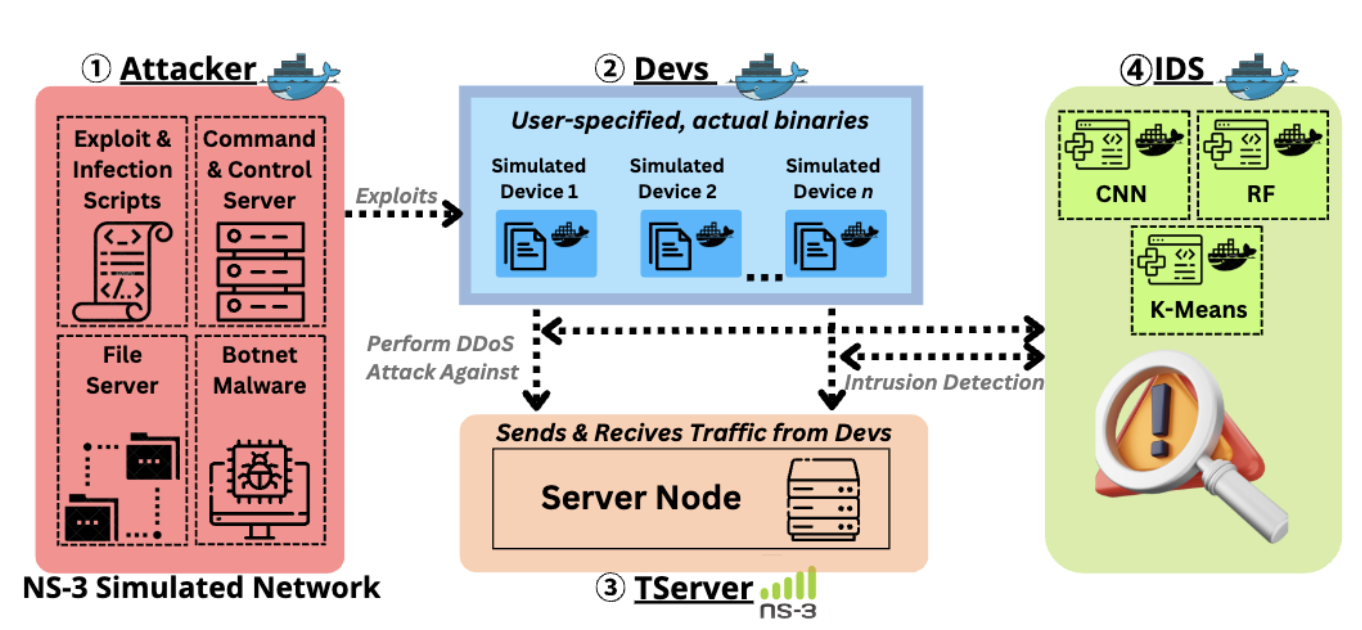
\includegraphics[scale= 0.6]{UNINA_MSc_Thesis_Project/img/chapterSimulatore/DDoShield.png}
  \caption{Architettura DDoShield}
\end{figure}


Questa architettura modulare consente di testare diverse configurazioni e scenari di attacco, rendendo DDoShield uno strumento flessibile e potente per la ricerca nel campo della sicurezza IoT.

Infine, oltre alla simulazione degli attacchi e alla valutazione delle prestazioni degli IDS in termini di accuratezza, DDoShield offre strumenti per misurare l'utilizzo delle risorse e la sostenibilità. Il tool è infatti in grado di rilevare metriche di performance degli IDS, come l'uso della CPU e della memoria, un aspetto cruciale quando si considera l'implementazione degli IDS in contesti IoT, dove i dispositivi hanno risorse limitate.

La valutazione delle prestazioni avviene in due fasi principali:
\begin{enumerate}
    \item \textbf{Fase di addestramento}: In questa fase, i modelli di machine learning sono addestrati su un dataset generato da DDoShield, che include sia traffico benigno che malevolo. I modelli vengono valutati in base a metriche come l'accuratezza, la precisione, il recall e l'F1-score. Durante questa fase, vengono anche misurate le risorse computazionali utilizzate per addestrare i modelli, in modo da determinare l'efficienza di ciascun algoritmo.
    \item \textbf{Fase di rilevamento in tempo reale}: Dopo l'addestramento, i modelli vengono utilizzati per rilevare attacchi in tempo reale durante la simulazione. Durante questa fase, DDoShield misura l'accuratezza del rilevamento, monitorando il tempo necessario per identificare un attacco e l'utilizzo delle risorse durante l'analisi del traffico di rete.
\end{enumerate}

Le metriche raccolte durante queste fasi offrono un quadro completo delle capacità del sistema IDS e permettono ai ricercatori di ottimizzare i modelli per ottenere il miglior compromesso tra accuratezza e utilizzo delle risorse. Per esempio, l'uso delle CNN può garantire una maggiore accuratezza nel rilevamento delle anomalie, ma al costo di un utilizzo di risorse computazionali più elevato rispetto ad altri modelli come il K-Means.
\cite{DDoShield}